\subsection{Masking (removing columns from) alignments with ssu-mask}
\label{sec:tutorial-masking}

If your goal is to use a phylogenetic inference program to build trees
from alignments created by \prog{ssu-align}, you should mask
out columns of the alignment that likely include a significant number
of misaligned nucleotides first, and then only run the inference on
the remaining columns where you're confident the alignment is correct. 

\begin{comment}
SSU alignments are commonly used for phylogenetic inference to
characterize the diversity of microorganisms in an environmental
sample. Because alignment errors confound phylogenetic inference, 
it is first recommended to remove columns from, or mask, SSU
alignments to remove regions that are likely to contain at least some
errors. 
\end{comment}

The \prog{ssu-mask} program uses the posterior probabilities
(PP values) in the alignments to determine which alignment columns
contain a significant fraction of nucleotides that are aligned with
low confidence. It takes a single command-line argument, the name of
the directory created by \prog{ssu-align}. The directory must exist
within the current working directory. To run it for our example, do: 

\user{ssu-mask myseqs} 

As with \prog{ssu-align}, the program will print information to the
screen about what it is doing and the files it is creating:

\begin{sreoutput}
# Masking alignments based on posterior probabilities...
#
#                                                    mask    
#                                                ------------
# file name                 in/out  type  #cols  incl.  excl.
# ------------------------  ------  ----  -----  -----  -----
  myseqs.archaea.stk         input   aln   1511      -      -
  myseqs.archaea.mask       output  mask   1508   1449     59
  myseqs.archaea.mask.pdf   output   pdf   1508   1449     59
  myseqs.archaea.mask.stk   output   aln   1449      -      -
#
  myseqs.bacteria.stk        input   aln   1597      -      -
  myseqs.bacteria.mask      output  mask   1582   1499     83
  myseqs.bacteria.mask.pdf  output   pdf   1582   1499     83
  myseqs.bacteria.mask.stk  output   aln   1499      -      -
#
  myseqs.eukarya.stk         input   aln   2009      -      -
  myseqs.eukarya.mask       output  mask   1881   1634    247
  myseqs.eukarya.mask.pdf   output   pdf   1881   1634    247
  myseqs.eukarya.mask.stk   output   aln   1634      -      -
\end{sreoutput}

The \prog{file name} column includes file names, either input or
output files, as listed in the \prog{in/out} field, with type
specified by the \prog{type} column: \prog{aln} for alignment,
\prog{mask} for mask file, and \prog{pdf} or \prog{ps} for structure
diagram file. The \prog{cols} column gives the number of columns for the
file. The \prog{incl.} and \prog{excl.} columns list the number of consensus
columns of the alignment that are included (not removed) and excluded
(removed), respectively, by the mask. For example, the
\prog{myseqs.archaea.stk} input alignment was initially 1511 total
columns, 1508 of which were consensus columns and 3 of which were insert
columns; the 3 insert columns and 59 of the 1508 consensus columns
were deemed unreliable and removed by the mask based on the PP values
in those columns, the remaining 1449 were saved as a new alignment to
\prog{myseqs.archaea.mask.stk}.

Importantly, all insert columns are always removed by \prog{ssu-mask}
regardless of the PP values in those columns. This is because the
nucleotides in these columns are not actually aligned between
different sequences, but rather simply inserted between the
appropriate consensus columns in the alignment. 
See figure~\ref{fig:toyex} (page~\pageref{fig:toyex}) in
section~\ref{sec:background} for an example. Insert columns should
therefore be removed prior to phylogenetic analysis which assumes
all nucleotides in the same column are homologous. 

In addition to alignments, the command above has generated two more files
for each of the domains: 
mask file (e.g. \prog{myseqs.archaea.mask}), and a structure diagram file
showing the masked positions on the consensus secondary structure:
\prog{myseqs.archaea.mask.pdf} or
\prog{myseqs.archaea.mask.ps} \footnote{If the program \prog{ps2pdf} is
    in your PATH, a PDF will be created, otherwise a postscript
    \prog{.ps} suffixed file will be created.}.

The mask file is a single line of text of length 1508 characters, one per
consensus position, containing only \prog{0}s and \prog{1}s. 
A \prog{0} at position \emph{n} indicates that consensus position \emph{n}
was excluded when the mask was applied, and a \prog{1} at position
\emph{n} indicates that consensus position \emph{n} was kept and
included in \prog{myseqs.archaea.mask.stk}. In this mask file there are
1449 \prog{1s} and 59 \prog{0s}.

The secondary structure diagram file highlights which positions on the
consensus structure are excluded by the mask. The
\prog{myseqs.archaea.mask.pdf} is included in this guide
as figure~\ref{fig:myseqs-archaea-mask}.

\begin{figure}
  \begin{center}
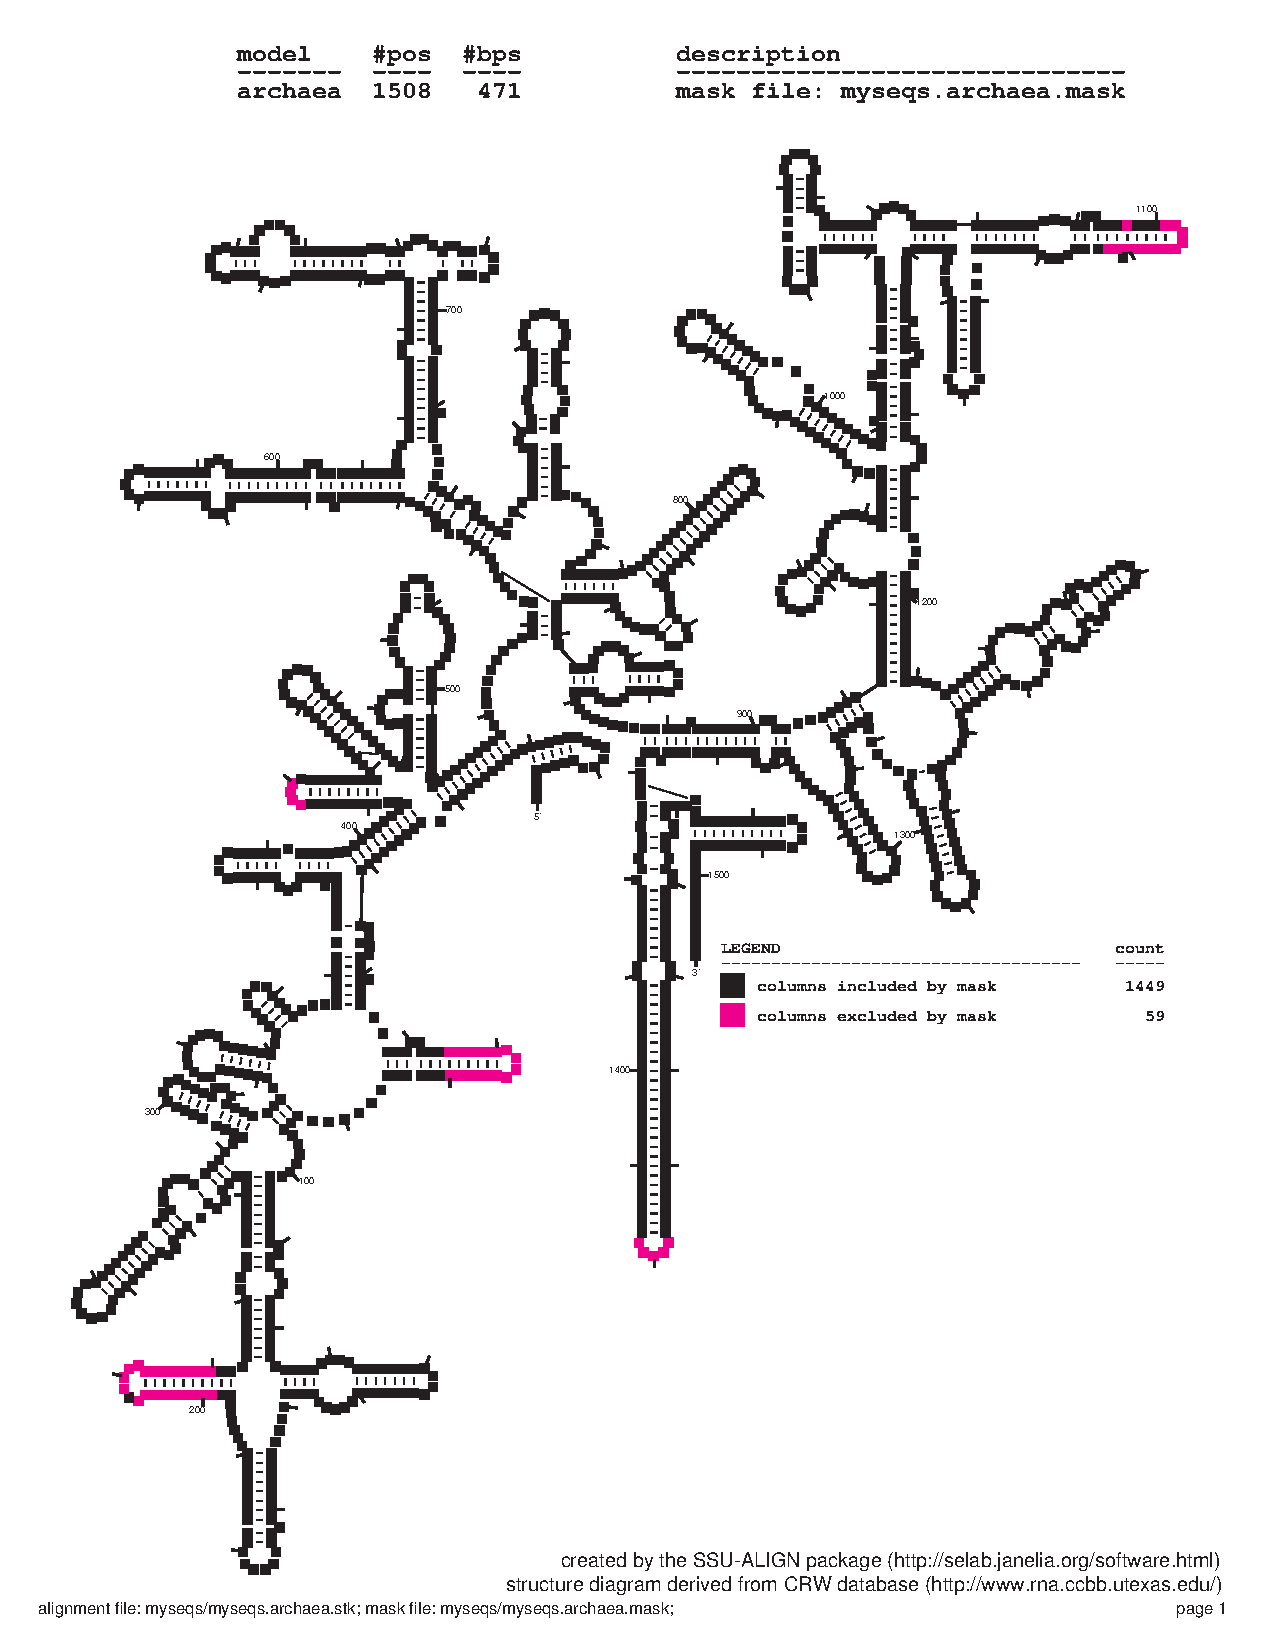
\includegraphics[width=5.7in]{Figures/myseqs-archaea-mask}
  \end{center}
\caption{\textbf{Archaeal posterior probability-based mask for the
    tutorial example.}
  Pink positions are excluded by the mask. Black positions are
  included.}
\label{fig:myseqs-archaea-mask}
\end{figure}

\subsubsection{Using precalculated masks for consistent masking of
  multiple datasets}

In the \prog{ssu-mask} example above, we calculated a mask
specifically based on our \prog{myseqs} alignments. Given a different
dataset of SSU sequences, the generated masks would likely be
different (i.e. exclude different columns). This
per-alignment-specificity can be undesirable. For example, if you'd
like to directly compare alignments from multiple runs of
\prog{ssu-align} you probably want to make sure all of the
alignments being compared contain an identical set of consensus
positions \footnote{This would also allow the alignments to be combined
easily; see the \prog{ssu-merge} manual page.}. SSU-ALIGN
contains a default, precalculated mask for each of the three
models. These masks were derived from large alignments as
described in section~\ref{sec:masks}. As we'll see in the next example, you
can use these masks by supplying the \prog{-d} option to
\prog{ssu-mask}. We'll also use the \prog{--key-out} option to add the
string ``default'' to the names of the output files so we do not
overwrite the files we created in the previous example. This option
enables you to save multiple sets of alignments and masks in a single
directory:

\user{ssu-mask -d --key-out default myseqs}

\begin{sreoutput}
# Masking alignments using pre-existing masks...
#
#                                                    mask    
#                                                ------------
# file name                 in/out  type  #cols  incl.  excl.
# ------------------------  ------  ----  -----  -----  -----
  myseqs.archaea.stk         input   aln   1511      -      -
  archaea-0p1.mask           input  mask   1508   1376    132
  myseqs.archaea.mask.pdf   output   pdf   1508   1376    132
  myseqs.archaea.mask.stk   output   aln   1376      -      -
#
  myseqs.bacteria.stk        input   aln   1597      -      -
  bacteria-0p1.mask          input  mask   1582   1376    206
  myseqs.bacteria.mask.pdf  output   pdf   1582   1376    206
  myseqs.bacteria.mask.stk  output   aln   1376      -      -
#
  myseqs.eukarya.stk         input   aln   2009      -      -
  eukarya-0p1.mask           input  mask   1881   1343    538
  myseqs.eukarya.mask.pdf   output   pdf   1881   1343    538
  myseqs.eukarya.mask.stk   output   aln   1343      -      -
\end{sreoutput}

The output is similar to the previous example, but note that the
\prog{.mask} suffixed files were input rather than output (these files
were placed in your \$SSUALIGNDIR directory during installation), and the number
of columns included and excluded has changed.

There are several other options that can be supplied to
\prog{ssu-mask}, including \prog{-s} and \prog{-k} which let you 
use your own precalculated masks. See the \prog{ssu-mask}
manual page at the end of this guide for more information. 

\subsubsection{Converting Stockholm alignments to FASTA format}
Once the ambiguously aligned regions of the alignment are removed you may
want to use the alignments as input to a phylogenetic inference
program. Not many of those programs accept Stockholm formatted
alignments as input. You can convert the Stockholm alignments to aligned FASTA
using the \prog{ssu-mask} program by specifying the \prog{--stk2afa}
option on the command line:

\user{ssu-mask --stk2afa myseqs}

After running, three \prog{.afa} suffixed files will have been created
in the \prog{myseqs} directory.




